\documentclass[12pt]{article}

\usepackage[utf8]{inputenc}
\usepackage{datetime}
\usepackage{amsthm}
\usepackage{amsmath}
\usepackage{amssymb}
\usepackage{enumitem}
\usepackage[USenglish]{babel}
\usepackage{matlab-prettifier}
\usepackage{graphicx}
\usepackage[makeroom]{cancel}
\usepackage{afterpage}
\usepackage{capt-of}
\usepackage{cite}
\usepackage{url}

\DeclareMathOperator*{\argmin}{arg\,min}
\DeclareMathOperator*{\argmax}{arg\,max}

\newcommand\independent{\protect\mathpalette{\protect\independenT}{\perp}}
\def\independenT#1#2{\mathrel{\rlap{$#1#2$}\mkern2mu{#1#2}}}

\newtheoremstyle{colon}{\topsep}{\topsep}{}{}{\bfseries}{:}{ }{}
\theoremstyle{colon}
\newtheorem{exercise}{Exercise}
\newtheorem*{answer}{Answer}

\title{ORFE 525: Statistical Learning and \\ Nonparametric Estimation \\ Project Literature Review}
\author{Zachary Hervieux-Moore}

\newdate{date}{18}{04}{2017}
\date{\displaydate{date}}

\begin{document}

\maketitle

\clearpage

\section{Introduction}

The problem that this project aims to address is that of classifying handwritten mathematical equations to its correct \emph{LaTeX} formulation. In fact, this is very similar to a request for research put out by Open AI \cite{openai}. A team from Harvard has submitted their solution on Open AI and has graciously provided their 100k image dataset \cite{1609.04938}. The techniques we wish to use to tackle this problem are modern neural network architectures such as the sequence-to-sequence model, a type of recurrent neural network (RNN), and generative adversarial networks (GAN). The proceeding sections aim to introduce these architectures and how they may be applied to this problem.

\section{Similar Research}

Alluded to above, one team has tackled a similar problem. The team had two goals, the first was to take images of compiled \emph{LaTeX} formulas and generate the original \emph{LaTeX}. The other was to take web pages and generate the HTML that rendered it. Both problems are similar as they involved decompiling an end result into an original markup language. The architecture they used was a combination of a convolutional neural network (CNN) to extract features from an image and then to use an sequence-to-sequence model architecture to allow for varying input and output sizes. Both these architectures are explored further in section 3. With this structure, they are able to achieve an exact match (correctly outputting \emph{LaTeX} that generates the image) rate of 75\% \cite{1609.04938}. A result which is extremely relevant to the problem at hand as the only change to the problem is the input from compiled \emph{LaTeX} images to handwritten equations. While a similar architecture as above may be used, differences in the convolutional layer may be beneficial to orient the network to extract features from handwriting as opposed to typeset formulas.

\clearpage

\section{Architectures}

\subsection*{Convolutional Neural Networks}

CNN's were covered in the class by Junwei and so not too much time will be spent here. What will be said is that CNN's have been used for a very long time for optical character recognition as exemplified by LeCun \textit{et al.} in \cite{lecun_bottou_bengio_haffner_1998}. Since then, there has been the introduction of max pooling, rectified linear units (ReLU), fully connected layers, among other variants. One merely has to look at any of the most successful neural networks in image recognition \cite{NIPS2012_4824}, \cite{szegedy2013deep}, text comprehension \cite{wang2012end}, or video classification \cite{karpathy2014large} to see an example of a modern day convolution neural network.

\subsection*{Recurrent Neural Networks}

Again, Junwei went over the basics of RNN's in class and so we skip the conversation to the state of the art architectures relevant to the application in mind. One clear problem that our neural network will face is turning images into arbitrary length pieces of \emph{LaTeX} code. Originally, RNN's only allowed for fixed length outputs. However, Cho \textit{et al.} introduced the sequence-to-sequence model in \cite{1406.1078} which allows for arbitrary input and output lengths. To understand how it works, Figure 1 displays the general architecture.
\begin{center}
  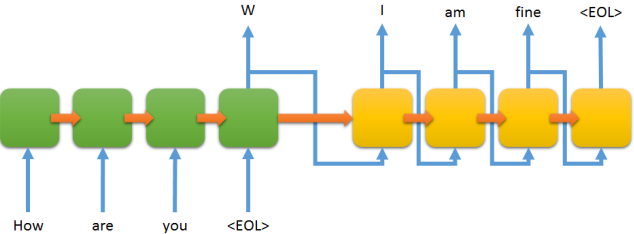
\includegraphics[width=0.8\textwidth]{sequence-to-sequence.png}
  \captionof{figure}{General Layout of a Sequence-to-Sequence Model \cite{seq2seq}}
\end{center}
First, there are two components of the network, the encoder (green) and decoder (yellow). How the network works is that the encoder is fed an arbitrary long input sequence until the sequence ends (denoted by \texttt{<EOL>}) above. Once the \texttt{<EOL>} is fed into the encoder, it produces an output. Now, the output is fed into the decoder and this is used to generate the output sequence (``I'' being the first output). This output then becomes the input and is fed until the decoder produces an \texttt{<EOL>} of its own. A prime example of this architecture  is used in translation \cite{1409.3215}.

One problem that arises with this architecture is that the encoder tends to not be able to learn long term behaviour. This is rectified by using Long Short Term Memory Cells (LSTM) which are the blocks in Figure 1. The details will be spared here, but the main idea is that you keep a state of the network along with the outputs and force the state to lose information (``forget'') about the previous state if it is not heavily weighted and replace this with information from the current input. For an in depth review of LSTM's and a comparison of its variants see \cite{1503.04069}.

Although the above sequence-to-sequence model works quite well, there is one potential deficiency. That is, in the step from the encoder to the decoder, the output of the encoder must be of a fixed length. Considering that the input is of variable length, this begs the question of whether or not the fixed length at the end diminishes the effect of learning from an arbitrary sequence. This is the exact problem that Bahdanau \textit{et al.} attempt to solve in \cite{1409.0473}. Their proposed solution is a so-called attention mechanism. This essentially makes the network much more complicated by feeding all of the outputs from the encoder to be available at each input for the decoder. However, for the added complexity, one generally achieves better results and using the attention mechanism allows one to analyze how the network is weighting different inputs to get a better sense of how the network is working as described in the results section of \cite{1409.0473}.

\subsection*{Generative Adversarial Networks}

The last architecture we will mention is the generative adversarial network (GAN). The GAN is a very recent result from Goodfellow \textit{et al.} \cite{1406.2661}. In this paper, they create a model that allows for a trained network to generate ``fake'' data that resembles the training set given to the network. This is achieved by creating two agents, a discriminator, and a generator whose job it is to fool the other. That is, the discriminator is trained to detect fake input given by generator and the generator is trained to try and fool the discriminator. Mathematically, the objective is given in \cite{1406.2661} as
\begin{gather*}
  \min_G \max_D V(D,G) = \mathbb{E}_{x \sim p_{data} (x)} [\log D(x)] + \mathbb{E}_{x \sim p_z (z)} [\log (1-D(G(z)))] \
\end{gather*}
To see how GAN's might be useful for my application, consider the work in \cite{reed2016generative}. In this paper, the researchers create a GAN that is able to generate images of birds and flowers based on a descriptive text. While this is not particularly relevant, the part that is promising is that they are able to generate images from text descriptions that the network has never seen before. Consider flipping their network, that is, images to text descriptions. In my case, it would be \emph{LaTeX} equations, and training a GAN that outputs \emph{LaTeX} this way. The problem with this architecture is that it requires many examples of a specific class. Whereas, in my problem, we are given one equation and one label. Thus, we turn our attention to applications of GAN's for classification purposes.

One example of work done in the area of classification using GAN's is \cite{1511.06434}. In this paper, they use a GAN as a feature extractor and then use these features in a linear model (SVM in this case). With this, they are able to achieve results better than other modern unsupervised learning techniques but worse than some unsupervised CNN architectures. However, this is accomplished using half as many feature units which suggests that there is room for improvement with more computational power. In the same paper, the team accomplishes state of the art performance in another task. This demonstrates the promise of GAN's in classification. Again, the issue with these results with respect to handwriting to \emph{LaTeX} is that they depend on a small number of classes. By design, this problem has many different \emph{LaTeX} outputs and so these techniques cannot be applied directly.

\section{Conclusion}

To achieve the desired goal, the use of CNN's and RNN's seem necessary after reviewing the literature. However, there is potential for GAN's to be used in a novel way for classification. As this was a literature review, discussion of the implementation specifics was omitted but still important for the overall success of the project. These include data acquisition, data processing, training scheme, etc. All things considered, this is a very approachable problem and state of the art performance could be possible.

\clearpage

\bibliographystyle{ieeetr}
\bibliography{references.bib}

\end{document}